\documentclass[conference]{IEEEtran}

\usepackage{cite}
\usepackage{graphicx}
\usepackage{amsmath}
\usepackage{url}
\usepackage{booktabs}
\usepackage{xcolor}

\begin{document}

\title{Building VHDL Processors with Claude Code:\\From 16-Bit to 64-Bit FPU}

\author{
  \IEEEauthorblockN{George Teifel\textsuperscript{1,*}, Siamak Tavakoli\textsuperscript{1}}
  \IEEEauthorblockA{\textsuperscript{1}\textit{Department of Electrical and Computer Engineering,
  University of New Mexico}\\
  Albuquerque, NM 87131, USA\\
  \textsuperscript{*}gteifel@unm.edu}
}

\maketitle

\begin{abstract}
Manual design of register-transfer level (RTL) hardware descriptions remains a labor-intensive process requiring deep expertise in both digital logic and synthesis tool chains. This paper presents a skill-based methodology for AI-assisted hardware description language (HDL) generation using Claude Code, an AI coding assistant. A custom skill was constructed by merging two community-contributed FPGA design skills and augmenting them with three capabilities: a simulation-first test-driven development (TDD) mandate, live documentation retrieval via Context7 MCP integration, and Vivado version-aware code generation. Using this skill, six complete RISC-V processor designs were generated in a single session: three in Verilog and three in VHDL, spanning 16-bit educational cores (RV32I subset), 64-bit integer processors (RV64I), and a 64-bit processor with a full IEEE 754 double-precision floating-point unit (RV64IFD). The most complex design implements 68 instructions across 28 FPU operations in a 5-stage pipeline, consuming 12,969 look-up tables (LUTs) and 18 DSP48E1 slices on a Xilinx Artix-7 XC7A35T. The simulation-first verification approach identified 10 floating-point bugs in the initial generation and drove a 48\% reduction in LUT utilization, from approximately 25,000 to 12,969 LUTs. Formal verification using SystemVerilog Assertions with SymbiYosys bounded model checking was subsequently integrated, mathematically proving correctness properties for ALU operations, FPU IEEE 754 special-value handling, pipeline hazard detection, and memory bus protocols across all three processor variants. All designs were verified on a Digilent Basys~3 development board. The results suggest that domain-specific skill engineering can substantially improve the quality and completeness of AI-generated HDL.
\end{abstract}

% ─────────────────────────────────────────────────────────────────────
% I. INTRODUCTION
% ─────────────────────────────────────────────────────────────────────
\section{Introduction}

The design of digital processors at the register-transfer level demands simultaneous expertise in computer architecture, hardware description languages, synthesis tool chains, and verification methodology. Even experienced engineers require weeks to months to produce a verified processor design targeting a specific FPGA platform~\cite{patterson2017cod}. Recent advances in large language models (LLMs) have demonstrated promising capabilities in software code generation, but their application to hardware description languages remains largely exploratory, and prior results have been confined to small-scale designs~\cite{thakur2023date, blocklove2023chipchat, pearce2020dave, sun2024hdlgen, zhao2025resbench}.

The gap between LLM-generated HDL and practical processor design remains vast. Thakur et al.~\cite{thakur2023date} benchmarked LLMs on small Verilog module tasks at DATE 2023, reporting that the best model achieved only 25.9\% syntactically correct code and a mere 6.5\% functional correctness rate --- and these benchmarks targeted isolated modules such as counters, adders, and FIFOs, not complete processors. Pearce et al.~\cite{pearce2020dave} established early baselines at MLCAD 2020 with DAVE, which derived small Verilog modules from English descriptions but did not attempt system-level designs. Blocklove et al.~\cite{blocklove2023chipchat} achieved the most ambitious prior result at MLCAD 2023 with Chip-Chat, generating an 8-bit accumulator-based microprocessor that was claimed as the world's first wholly AI-written HDL for tapeout --- but it featured an 8-bit datapath, no pipeline, no floating-point unit, and a minimal instruction set. More recently, Sun et al.~\cite{sun2024hdlgen} used ChatGPT-3.5 to generate an RV32I processor in VHDL and Verilog, but the design was limited to 32-bit integer operations with no FPU and no dual-language parity. Zhao et al.~\cite{zhao2025resbench} introduced ResBench with 56 FPGA benchmarks measuring resource efficiency of LLM-generated designs, but these remained module-level benchmarks rather than complete processors.

This paper presents a fundamentally different approach that produces results exceeding prior work by orders of magnitude in complexity. Rather than improving the language model itself, the proposed methodology engineers the context in which the model operates. A custom skill for Claude Code~\cite{anthropic2026claude} was constructed to encode FPGA design expertise, enforce a simulation-first verification workflow, and provide access to live documentation through the Context7 Model Context Protocol (MCP). Using this skill, six complete RISC-V~\cite{waterman2019riscv} processor designs were generated in a single session, verified in simulation, and validated on physical hardware. The most complex design --- a 64-bit RV64IFD processor with a full IEEE 754 double-precision FPU implementing 68 instructions across 8 execution units in a 5-stage pipeline --- consumes 12,969 LUTs and 18 DSP48E1 slices on a Xilinx Artix-7, with dual-language output in both Verilog and VHDL. To the best of our knowledge, this represents the most complex processor design generated by a large language model to date, exceeding prior work by orders of magnitude in instruction count, datapath width, and functional unit complexity.

The contributions of this paper are threefold. First, a skill architecture is presented that merges community-contributed FPGA design knowledge with simulation-driven verification, live documentation retrieval, and synthesis tool version awareness. Second, a three-level testbench hierarchy is described that adapts test-driven development principles to hardware verification, catching 10 floating-point bugs and driving a 48\% reduction in resource utilization. Third, quantitative results are reported for six processor variants targeting the Xilinx Artix-7 XC7A35T~\cite{xilinx2020ds180}, including a 64-bit RV64IFD processor with a complete IEEE 754~\cite{ieee754_2019} double-precision floating-point unit consuming 12,969 LUTs.

% ─────────────────────────────────────────────────────────────────────
% II. METHODOLOGY
% ─────────────────────────────────────────────────────────────────────
\section{Methodology}

\subsection{Custom Skill Architecture}

The skill-based approach begins with the observation that LLM performance on domain-specific tasks depends critically on the context provided at generation time. Claude Code supports user-defined skills: structured context documents that prime the model with domain expertise, coding conventions, and workflow constraints before any code generation occurs. The custom FPGA skill used in this work was constructed by merging two existing community-contributed skills and augmenting them with three additional capabilities.

The first source skill focused on RTL design patterns: clock-domain crossing synchronizers, finite state machine (FSM) templates, block RAM (BRAM) inference rules, pipeline design heuristics, and DSP48E1 utilization strategies for Xilinx 7-series devices~\cite{xilinx2020ds180}. The second source skill centered on the Vivado~\cite{xilinx2020ug901} synthesis workflow: project creation via TCL scripting, synthesis and implementation settings, timing constraint idioms, and bitstream generation procedures. Neither skill was complete in isolation. A skill that encodes pipeline design patterns but lacks verification infrastructure produces code that may synthesize but cannot be validated. Conversely, a skill that automates the Vivado workflow but has no opinion on RTL structure will accept structurally deficient designs without objection.

The merged skill was augmented with three capabilities. First, a simulation-first TDD mandate was embedded as a hard constraint: the skill requires that every RTL module be accompanied by a self-checking testbench with explicit pass/fail assertions before synthesis is permitted. Second, Context7 MCP integration was added to enable live documentation retrieval. Rather than relying on the model's training data for RISC-V instruction encodings~\cite{waterman2019riscv}, IEEE 754 special-case rules~\cite{ieee754_2019}, or Vivado TCL syntax~\cite{xilinx2020ug901}, the skill queries authoritative sources at generation time. Third, Vivado version awareness was implemented to adapt generated code to the user's specific synthesis tool version. The skill detects the installed Vivado version and adjusts its output accordingly, avoiding incompatible TCL syntax, unsupported SystemVerilog constructs, and inappropriate device primitive instantiations.

The skill includes three reference files that ground every generation: \texttt{patterns.md} encodes structural design patterns, \texttt{sharp\_edges.md} catalogs known failure modes and their mitigations, and \texttt{validations.md} provides regex-based lint rules for common HDL errors such as incomplete sensitivity lists and unregistered outputs.

\subsection{Simulation-First Verification Framework}

The verification framework enforces a three-level testbench hierarchy adapted from software TDD principles. At the unit level, individual modules such as the ALU and each FPU execution unit are tested with known input/output vectors and IEEE 754 test constants. At the integration level, multi-module assemblies are verified by loading test programs via \texttt{\$readmemh} and checking register file state and program counter progression across instruction sequences. At the system level, complete processor instances execute test programs for thousands of simulation cycles, with results mapped to GPIO outputs for hardware correlation.

This hierarchy ensures that bugs are caught at the lowest possible level, where diagnosis is cheapest. Hardware bugs that escape to synthesis consume hours of place-and-route time and produce failures that are difficult to diagnose on physical devices. Catching those same bugs in simulation costs seconds. The skill makes simulation the mandatory first step, not an optional afterthought. Fig.~\ref{fig:tdd} illustrates this workflow.

\begin{figure}[t]
  \centering
  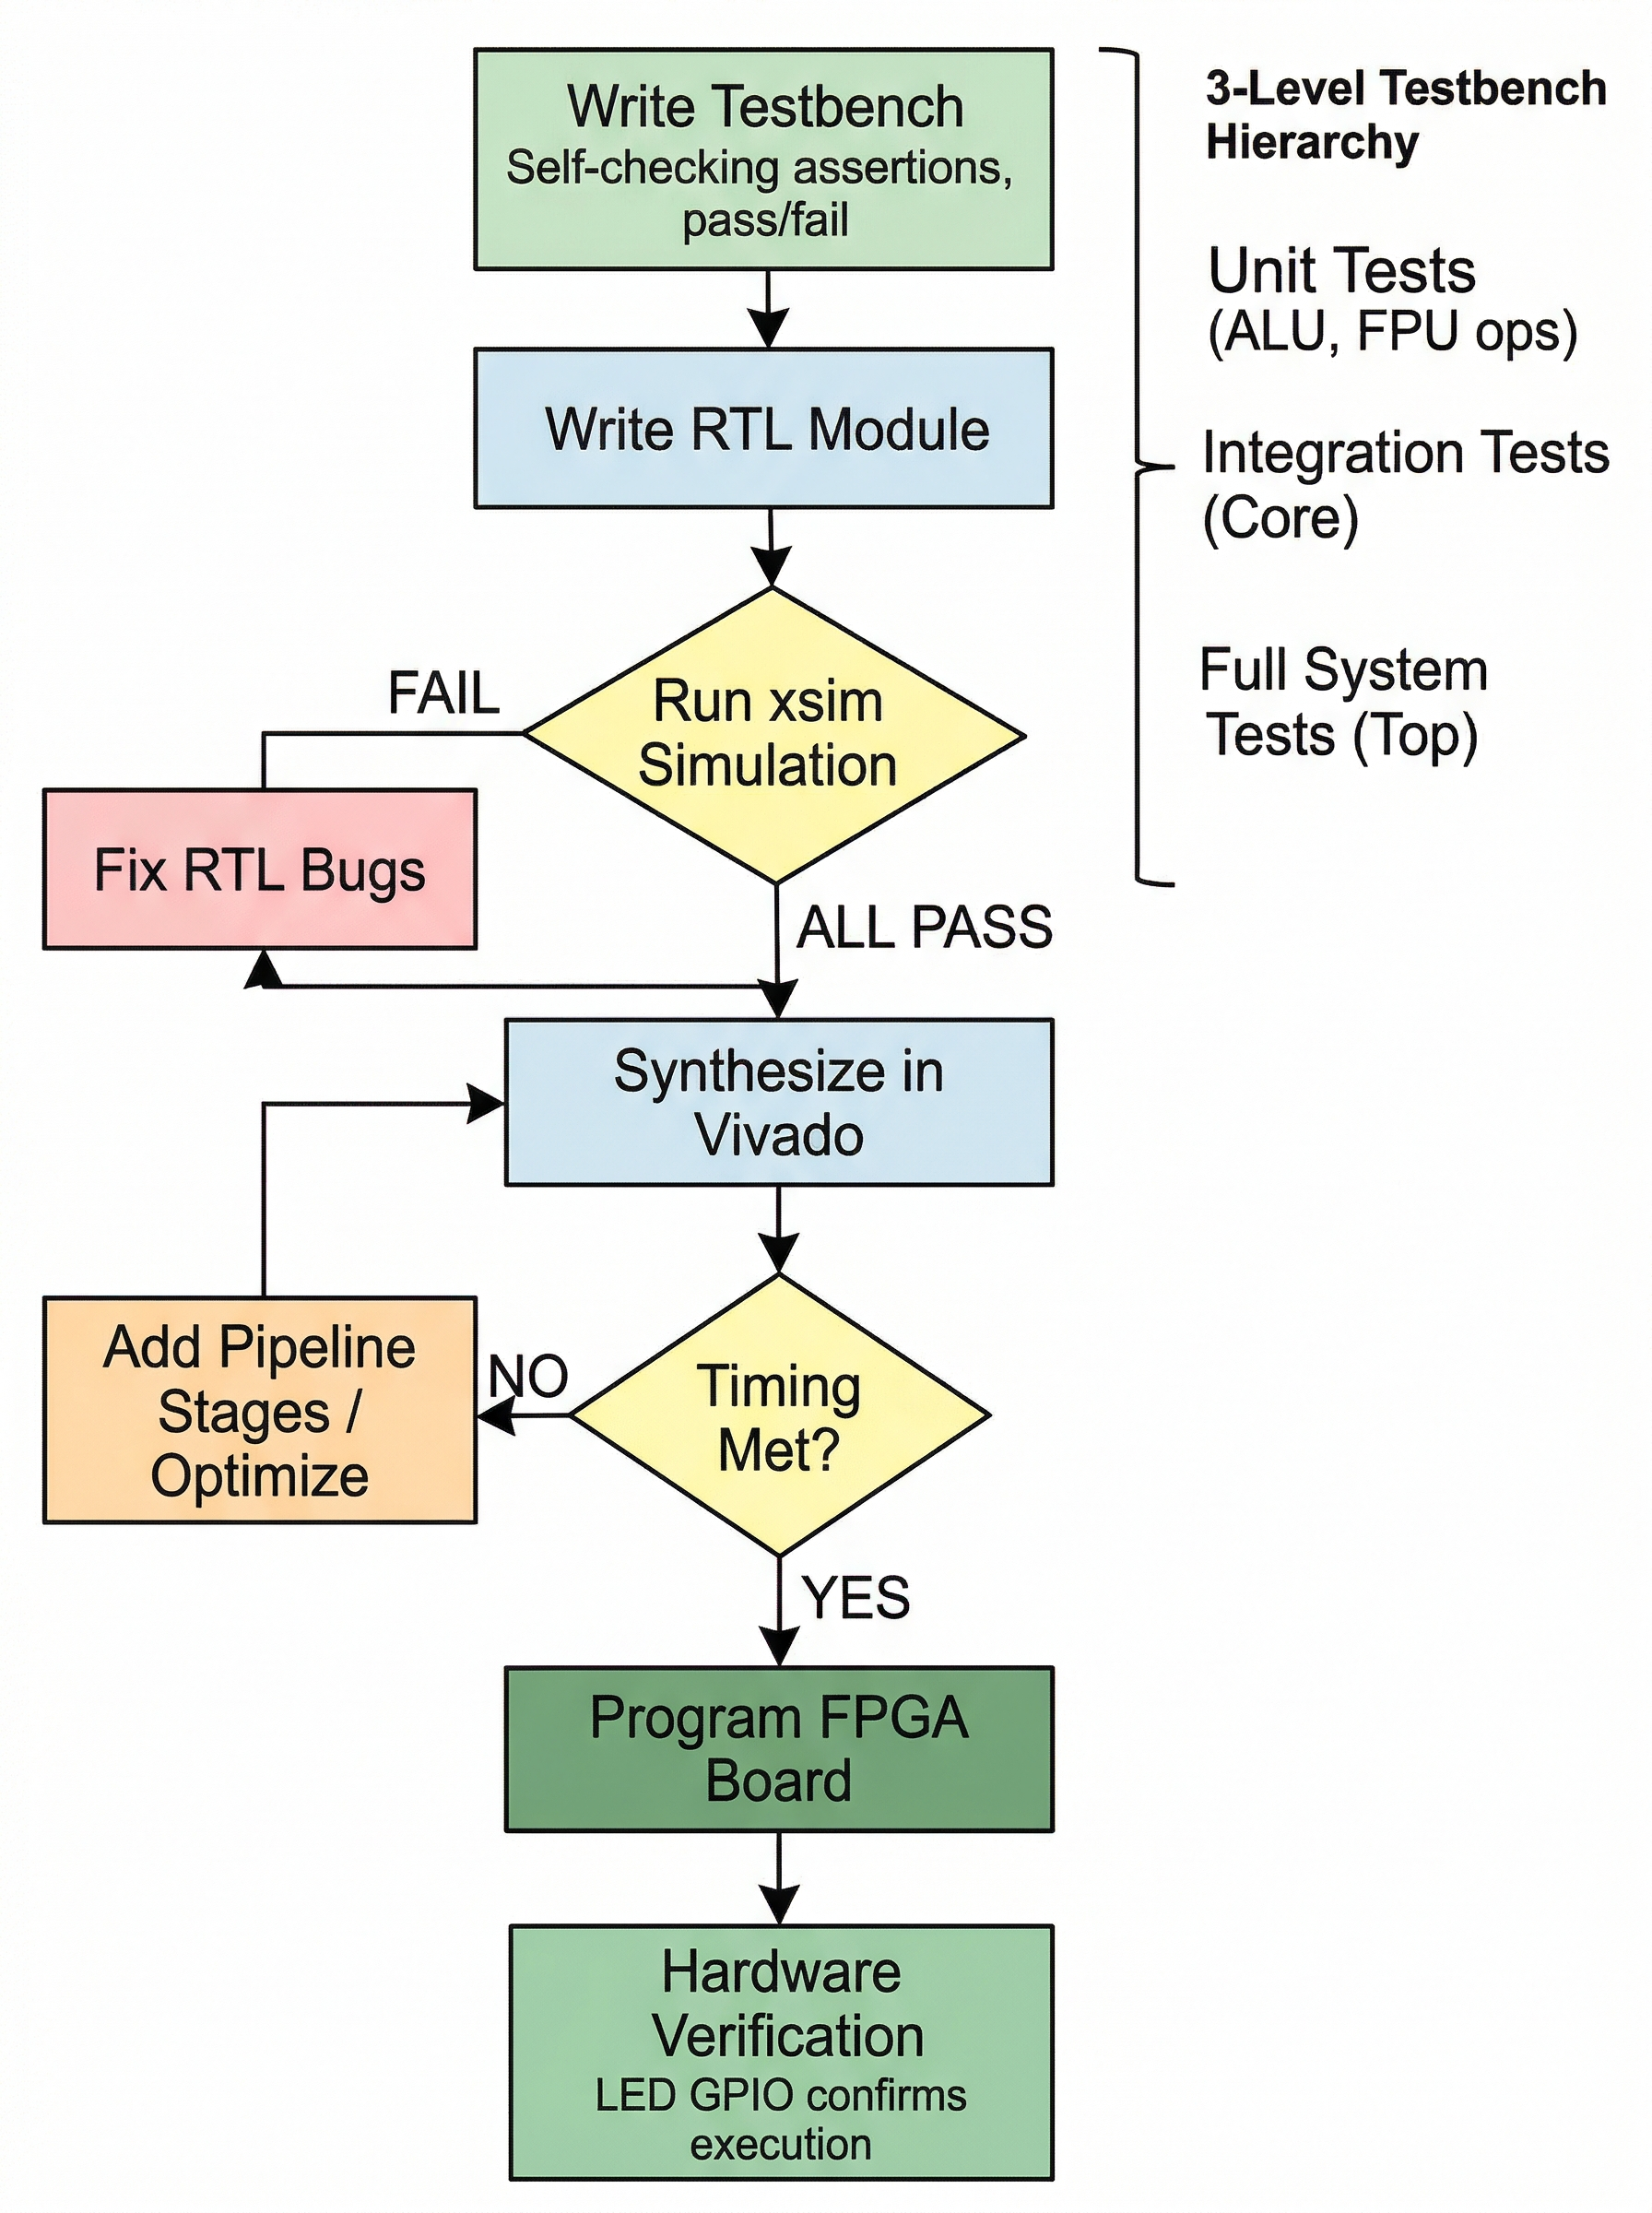
\includegraphics[width=0.85\columnwidth]{figures/fig_tdd_flow.jpg}
  \caption{Simulation-first verification workflow enforced by the custom FPGA skill.}
  \label{fig:tdd}
\end{figure}

\subsection{Target Platform}

All designs target the Digilent Basys~3 development board~\cite{digilent2021basys3}, which features a Xilinx Artix-7 XC7A35T-1CPG236C FPGA. This device provides 20,800 LUTs, 41,600 flip-flops, 90 DSP48E1 slices, and 50 36Kb block RAMs~\cite{xilinx2020ds180}. Synthesis, implementation, and bitstream generation were performed using Xilinx Vivado 2020.2~\cite{xilinx2020ug901}. The board operates at a native 100\,MHz clock frequency. Hardware verification employed the 16-LED array available on the Basys~3 through memory-mapped GPIO.

\subsection{Formal Verification Methodology}

To complement simulation-based testing, formal verification using SystemVerilog Assertions (SVA) was integrated into the verification infrastructure. While simulation provides coverage-based confidence through specific test vectors, formal verification employs satisfiability modulo theories (SMT) solvers to mathematically prove that design properties hold for all possible input combinations within a bounded number of clock cycles~\cite{wolf2016symbiyosys}. The two approaches are complementary: simulation catches functional bugs rapidly at low cost, while formal verification proves the absence of specific classes of bugs within the bounded depth.

The formal verification infrastructure comprises 16 SVA modules totaling approximately 1,500 lines of assertion code, organized into six property categories: (1)~protocol correctness, verifying handshake busy/done sequencing and timing bounds; (2)~ALU functional correctness, checking combinational operation results; (3)~FPU IEEE 754 special-value handling, verifying correct behavior for infinity, NaN, zero, and subnormal operands~\cite{ieee754_2019}; (4)~pipeline forwarding and hazard detection, confirming forwarding priority ordering (EX~$>$~MEM~$>$~WB) and the x0 hardwire invariant~\cite{waterman2019riscv}; (5)~reset synchronizer timing, proving dual-flip-flop metastability synchronizer invariants; and (6)~memory bus protocol, verifying address decode mutual exclusion and valid/ready handshaking.

A key design decision was the use of SystemVerilog \texttt{bind} statements to attach assertion modules to RTL without modifying the generated source code~\cite{ieee1800_2017}. This separation of concerns keeps the RTL clean and allows either verification approach to operate independently. Two verification engines are supported: SymbiYosys with the Z3 SMT solver for open-source bounded model checking across eight configurations with depths ranging from 1~cycle (combinational ALU verification) to 120~cycles (multi-cycle FPU operations), and Vivado xsim for assertion checking during simulation. A Makefile orchestrates both flows, enabling one-command verification of all properties across all three processor variants.

% ─────────────────────────────────────────────────────────────────────
% III. IMPLEMENTATION
% ─────────────────────────────────────────────────────────────────────
\section{Implementation}

\subsection{Processor Architecture}

The generated processor family comprises three architectural tiers. The rv16 design implements a 16-bit datapath with a 3-stage pipeline supporting a 12-instruction subset of the RV32I base integer instruction set. The rv64 design scales to a 64-bit datapath with a 3-stage pipeline implementing the full 40-instruction RV64I specification. The rv64fp design, the most complex variant, implements a 5-stage pipeline (Fetch, Decode, Execute, Memory, Writeback) supporting the RV64IFD instruction set with 68 instructions.

The rv64fp pipeline implements full data forwarding to resolve read-after-write (RAW) hazards without stalls in the common case. A dedicated hazard detection unit monitors inter-stage register dependencies and inserts pipeline bubbles for load-use hazards that cannot be resolved through forwarding alone. The architecture employs a Harvard memory model with separate instruction and data BRAM, plus memory-mapped GPIO for LED output. Fig.~\ref{fig:pipeline} illustrates the pipeline architecture.

\begin{figure*}[t]
  \centering
  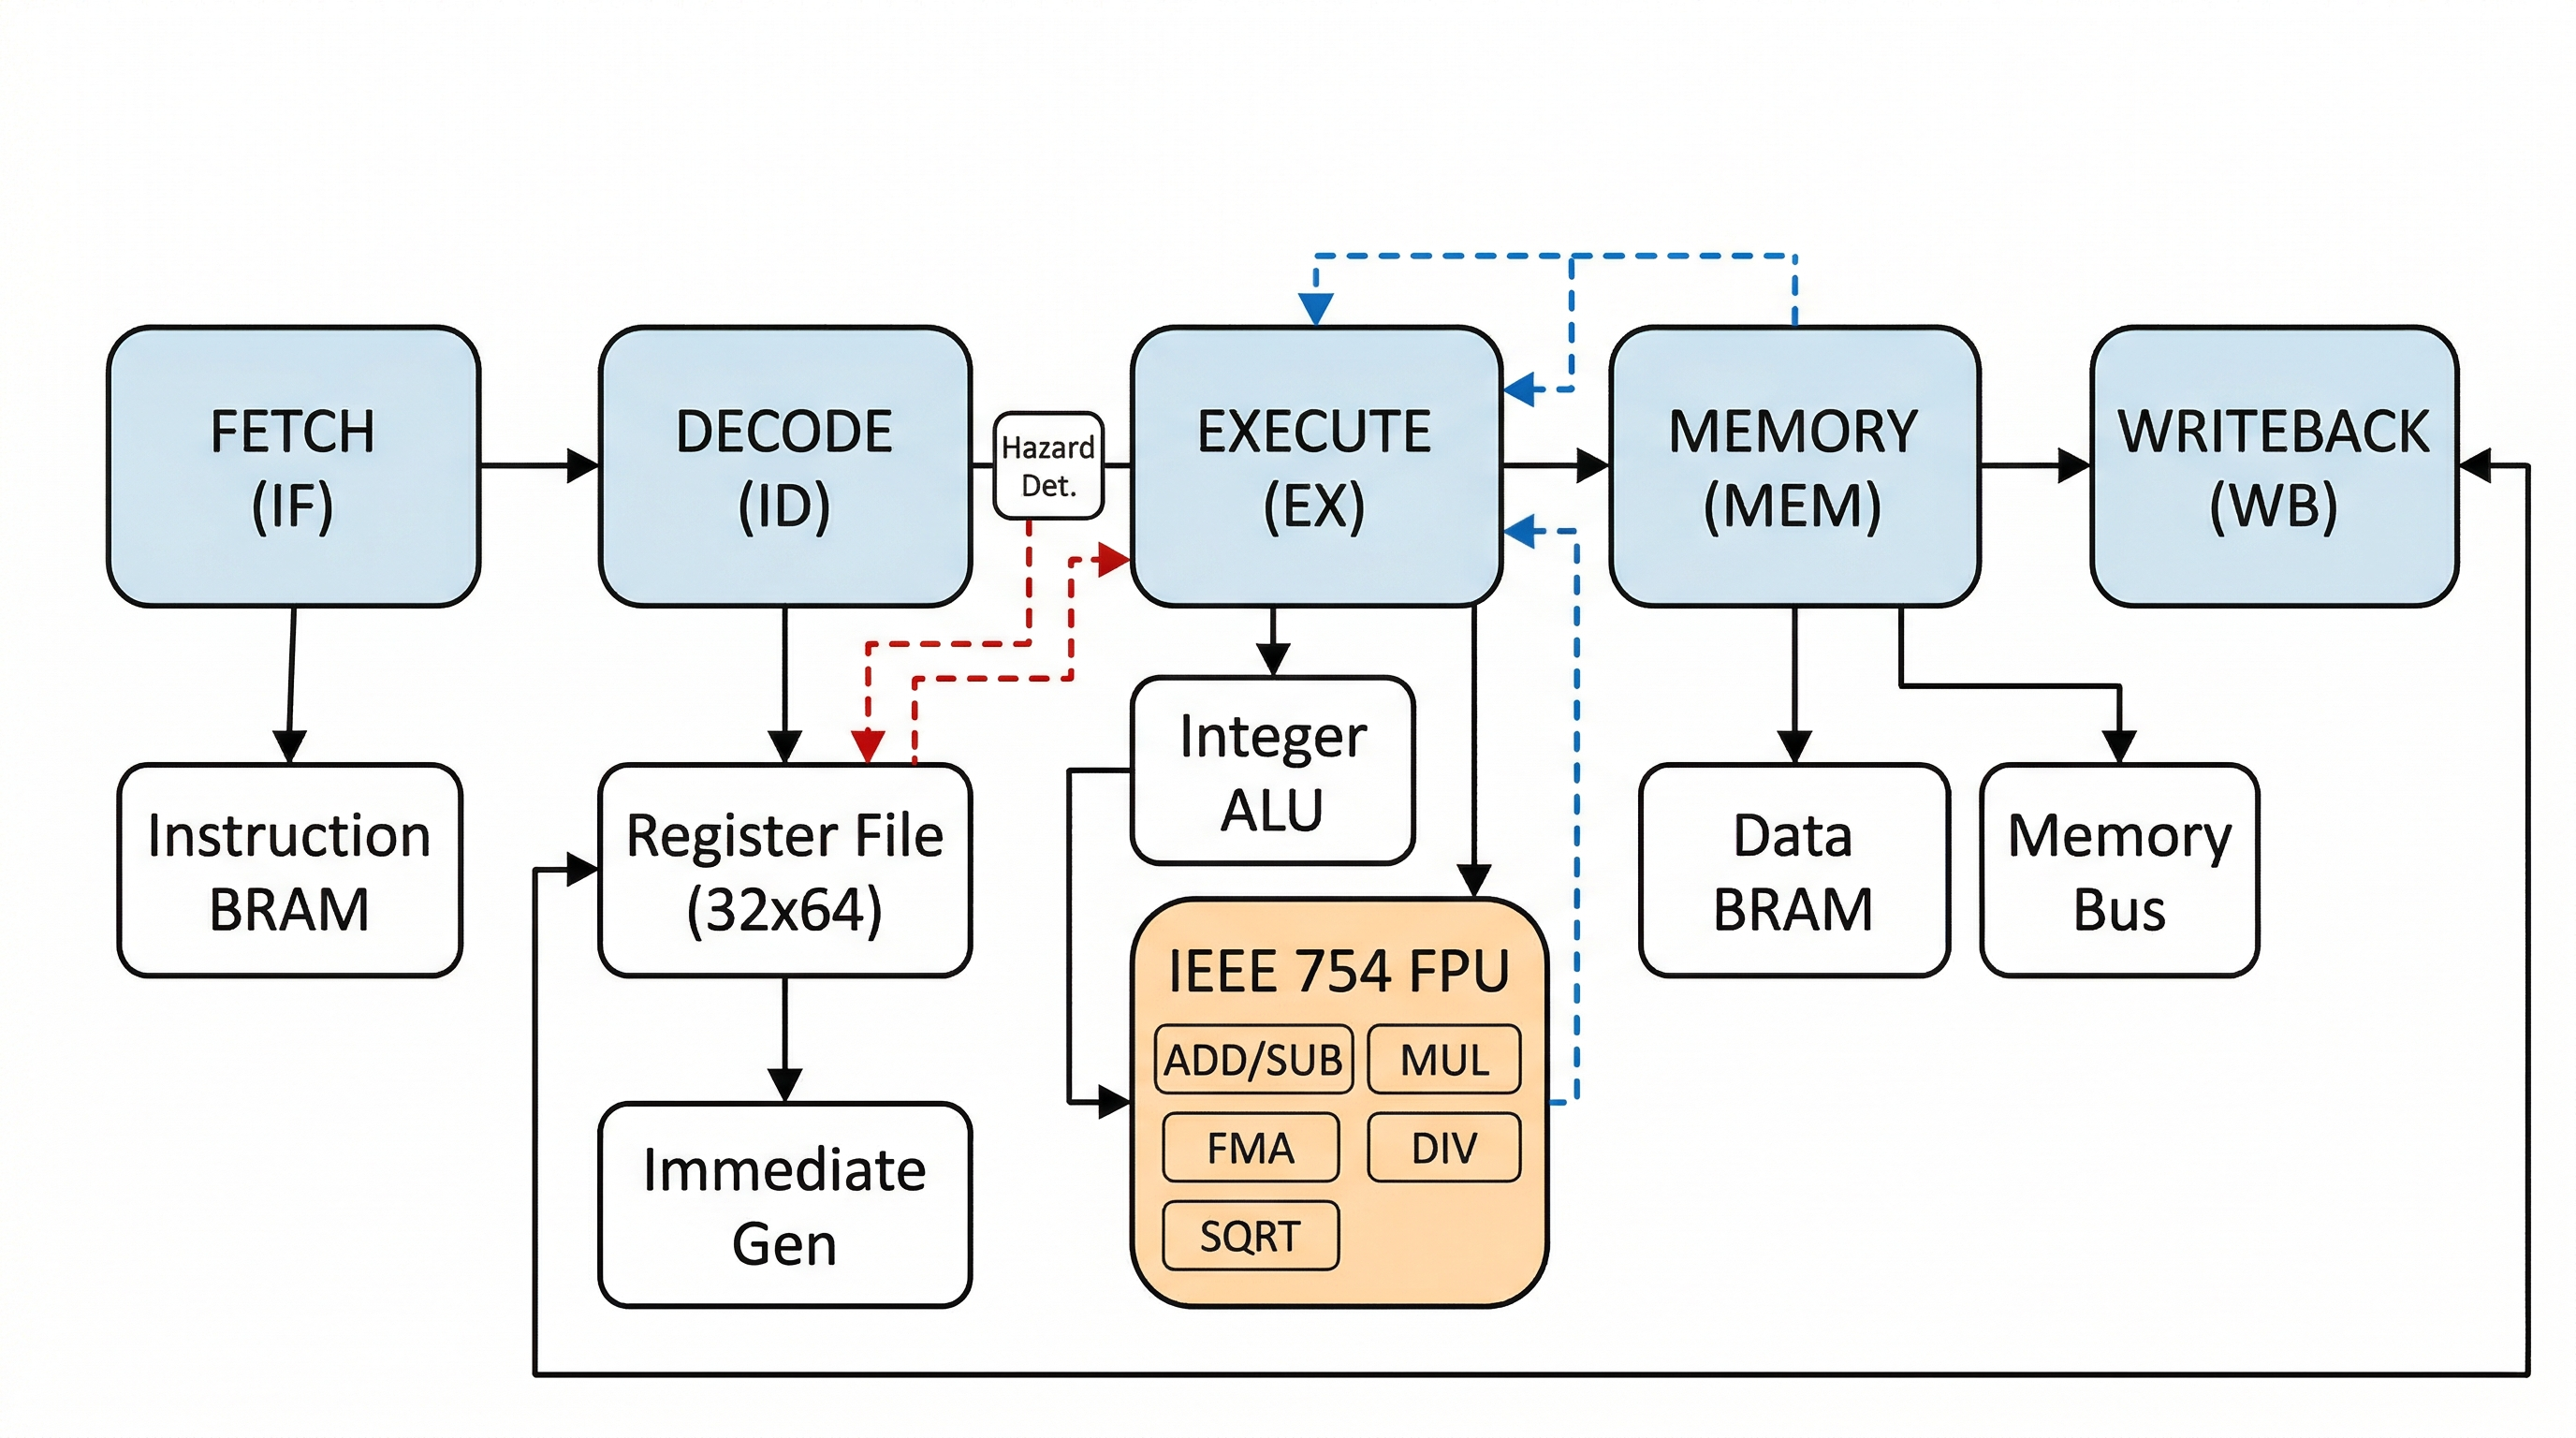
\includegraphics[width=\textwidth]{figures/fig_pipeline.jpg}
  \caption{Five-stage pipeline architecture of the rv64fp processor with IEEE 754 FPU.}
  \label{fig:pipeline}
\end{figure*}

\subsection{IEEE 754 Floating-Point Unit}

The floating-point unit implements 28 IEEE 754 double-precision operations~\cite{ieee754_2019} distributed across eight specialized execution units. The addition/subtraction unit employs a 3-cycle pipelined architecture with mantissa alignment shifting and leading-zero normalization. The multiplication unit uses a 3-cycle pipeline with DSP48E1 cascade~\cite{xilinx2020ds180} for full 53-by-53-bit mantissa multiplication. Fused multiply-add (FMA) operations, including FMADD, FMSUB, FNMSUB, and FNMADD, avoid intermediate rounding to achieve higher precision than sequential multiply-then-add operations. Division and square root are implemented as iterative multi-cycle units using digit-recurrence algorithms.

Additional operations include sign injection (FSGNJ, FSGNJN, FSGNJX), comparisons (FEQ, FLT, FLE) with proper NaN handling per IEEE 754, classification (FCLASS) for runtime type inspection, and format conversions (FCVT) between integer and floating-point representations in both directions. All five IEEE 754 rounding modes are supported: round to nearest even (RNE), round toward zero (RTZ), round down (RDN), round up (RUP), and round to nearest magnitude (RMM). Each execution unit independently handles special cases including NaN propagation, infinity arithmetic, signed zero, and subnormal numbers.

\subsection{Dual-Language Output}

Each processor variant was generated in both Verilog and VHDL, producing 26 RTL modules per language. The Verilog implementation totals 5,721 lines and the VHDL implementation totals 4,133 lines. Both language variants include complete Vivado TCL build scripts for project creation, synthesis, implementation, and bitstream generation, as well as shared Basys~3 constraint files (XDC format) for pin mapping and clock definition. Test programs were written in RISC-V assembly and compiled to hexadecimal memory initialization files via a Python assembler script.

% ─────────────────────────────────────────────────────────────────────
% IV. RESULTS
% ─────────────────────────────────────────────────────────────────────
\section{Results}

\subsection{Design Metrics}

Table~\ref{tab:metrics} summarizes the design metrics for all six processor variants. The designs span three orders of magnitude in complexity, from the 400-LUT rv16 educational core to the 12,969-LUT rv64fp processor with full floating-point support.

\begin{table}[t]
  \centering
  \caption{Design Metrics for All Processor Variants}
  \label{tab:metrics}
  \footnotesize
  \begin{tabular}{@{}lllllrl@{}}
    \toprule
    Processor & Lang. & Datapath & Pipeline & ISA & Instr. & LUTs \\
    \midrule
    rv16   & Verilog & 16-bit & 3-stage & RV32I sub. & 12 & $\sim$400 \\
    rv64   & Verilog & 64-bit & 3-stage & RV64I      & 40 & 3,273 \\
    rv64fp & Verilog & 64-bit & 5-stage & RV64IFD    & 68 & 12,969 \\
    rv16   & VHDL    & 16-bit & 3-stage & RV32I sub. & 12 & $\sim$400 \\
    rv64   & VHDL    & 64-bit & 3-stage & RV64I      & 40 & 3,273 \\
    rv64fp & VHDL    & 64-bit & 5-stage & RV64IFD    & 68 & 12,969 \\
    \bottomrule
  \end{tabular}
\end{table}

\subsection{Verification Results}

The simulation-first verification framework identified 10 bugs in the initial FPU generation. These included rounding edge cases in the addition/subtraction unit where guard, round, and sticky bit computation failed for specific mantissa alignment scenarios; NaN propagation errors in the comparison unit where quiet NaN and signaling NaN were not distinguished correctly per IEEE 754 Section~6.2~\cite{ieee754_2019}; and a sign bit inversion in the FNMSUB operation where the negation was applied to the wrong intermediate result.

Unit-level testbenches (\texttt{tb\_alu.v} and \texttt{tb\_fpu\_ops.v}) verified each ALU and FPU operation independently. The \texttt{tb\_fpu\_ops.v} testbench spans 327 lines and exercises all 28 FPU operations with IEEE 754 test constants including positive and negative zero, infinity, quiet NaN, signaling NaN, and subnormal values. Each test case includes a descriptive label for immediate failure identification in simulation logs, along with timeout protection to detect infinite loops in the iterative division and square root units.

Integration-level testbenches (\texttt{tb\_rv16\_core.v}) loaded test programs via \texttt{\$readmemh}, instantiated dual-port memory models, and verified program counter progression and register file state across multi-instruction sequences. These tests detected hazard detection failures and data forwarding bugs that unit-level testing alone could not reach. System-level testbenches (\texttt{tb\_rv64fp\_full.v}) executed complete test programs for over 2,000 simulation cycles and mapped FPU computation results to LED bit positions for correlation with hardware verification.

Formal verification using SymbiYosys bounded model checking proved correctness properties across all three processor variants. Table~\ref{tab:formal} summarizes the results by property category. For the rv64fp processor, bounded model checking to depth 120 proved FPU protocol correctness including the busy/done handshake invariant, eventual completion within bounded cycles, and IEEE 754 special-value handling for all five arithmetic operations. ALU properties were proven at depth~1 through combinational verification. Pipeline hazard detection properties confirmed forwarding priority ordering and the x0 hardwire invariant at depth~10. Memory bus properties verified address decode mutual exclusion and valid/ready protocol compliance.

The formal verification process confirmed the absence of protocol violations reachable within the bounded depths, providing stronger assurance than simulation alone. In particular, the FPU IEEE 754 properties verified correct NaN propagation, infinity arithmetic, and exception flag generation for edge cases that would require impractically large simulation test suites to exercise exhaustively. The \texttt{bind} methodology enabled formal verification to be added without modifying any of the 26 RTL modules per language, preserving the integrity of the simulation-verified designs.

\begin{table}[t]
  \centering
  \caption{Formal Verification Results by Property Category}
  \label{tab:formal}
  \footnotesize
  \begin{tabular}{@{}llllc@{}}
    \toprule
    Property Category & Variants & Engine & Depth & Status \\
    \midrule
    ALU Correctness     & rv16, rv64, rv64fp & SBY BMC & 1   & PASS \\
    FPU Protocol        & rv64fp             & SBY BMC & 120 & PASS \\
    FPU IEEE 754        & rv64fp             & SBY BMC & 120 & PASS \\
    Hazard Detection    & rv64fp             & SBY BMC & 10  & PASS \\
    Reset Synchronizer  & rv16, rv64, rv64fp & SBY BMC & 10  & PASS \\
    Memory Bus Protocol & rv64fp             & SBY BMC & 10  & PASS \\
    \bottomrule
  \end{tabular}
\end{table}

\begin{figure*}[t]
  \centering
  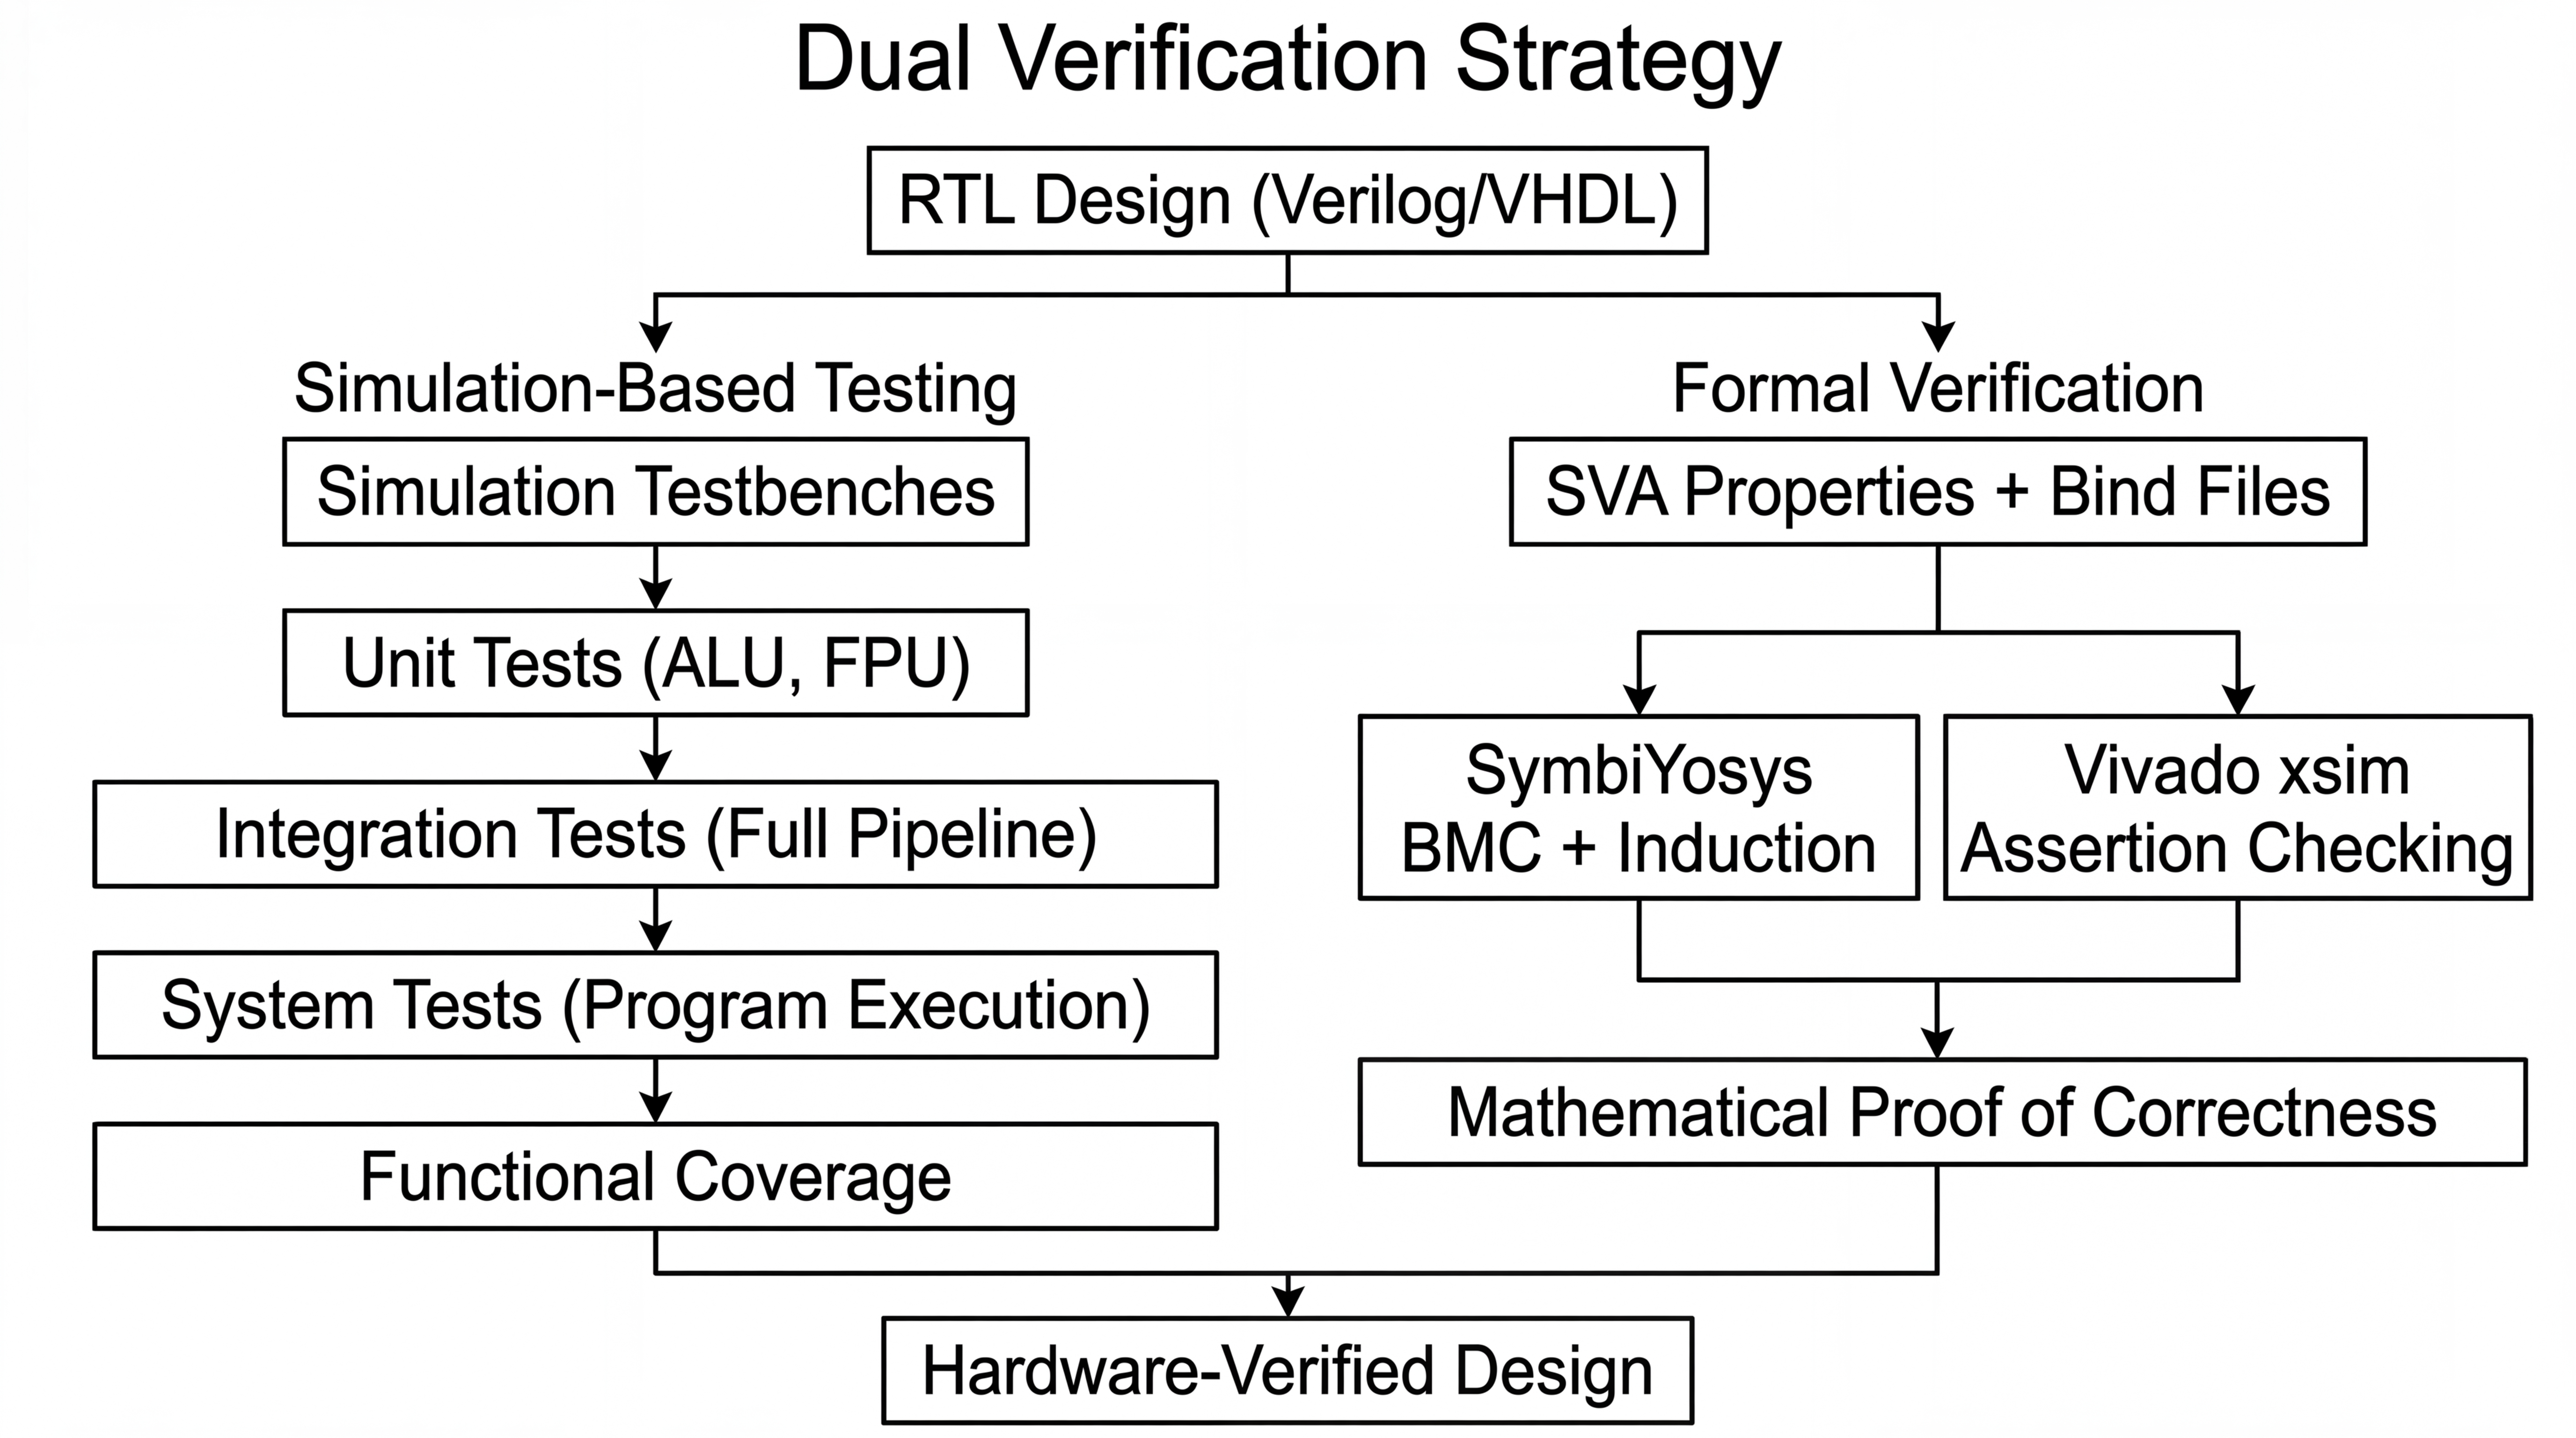
\includegraphics[width=\textwidth]{figures/fig_verification_strategy.jpg}
  \caption{Complementary verification strategy combining simulation-based testing and SVA formal verification.}
  \label{fig:verification}
\end{figure*}

\subsection{Resource Optimization}

The simulation-driven verification process produced a substantial reduction in resource utilization. The \texttt{fp\_fma} module, which implements fused multiply-add operations, was reduced from 13,932 LUTs to 1,942 LUTs, an 86\% reduction. The full rv64fp system decreased from approximately 25,000 LUTs to 12,969 LUTs, a 48\% overall reduction. Fig.~\ref{fig:lut} illustrates the LUT utilization before and after optimization.

This optimization was not the result of explicit resource minimization techniques. Rather, it was a natural consequence of the simulation-first methodology. When testbenches clarified the exact functional requirements for each module, dead logic paths and redundant special-case handling were identified and removed. The FMA unit, for example, contained elaborate exception handling code for cases that were already handled by upstream modules. Once simulation confirmed that these cases could not reach the FMA unit, the redundant logic was eliminated.

The final rv64fp design consumes 12,969 of the 20,800 available LUTs on the XC7A35T, representing 82.9\% utilization. The design also uses 18 of the 90 available DSP48E1 slices for mantissa multiplication in the floating-point multiplier and FMA units.

\begin{figure}[t]
  \centering
  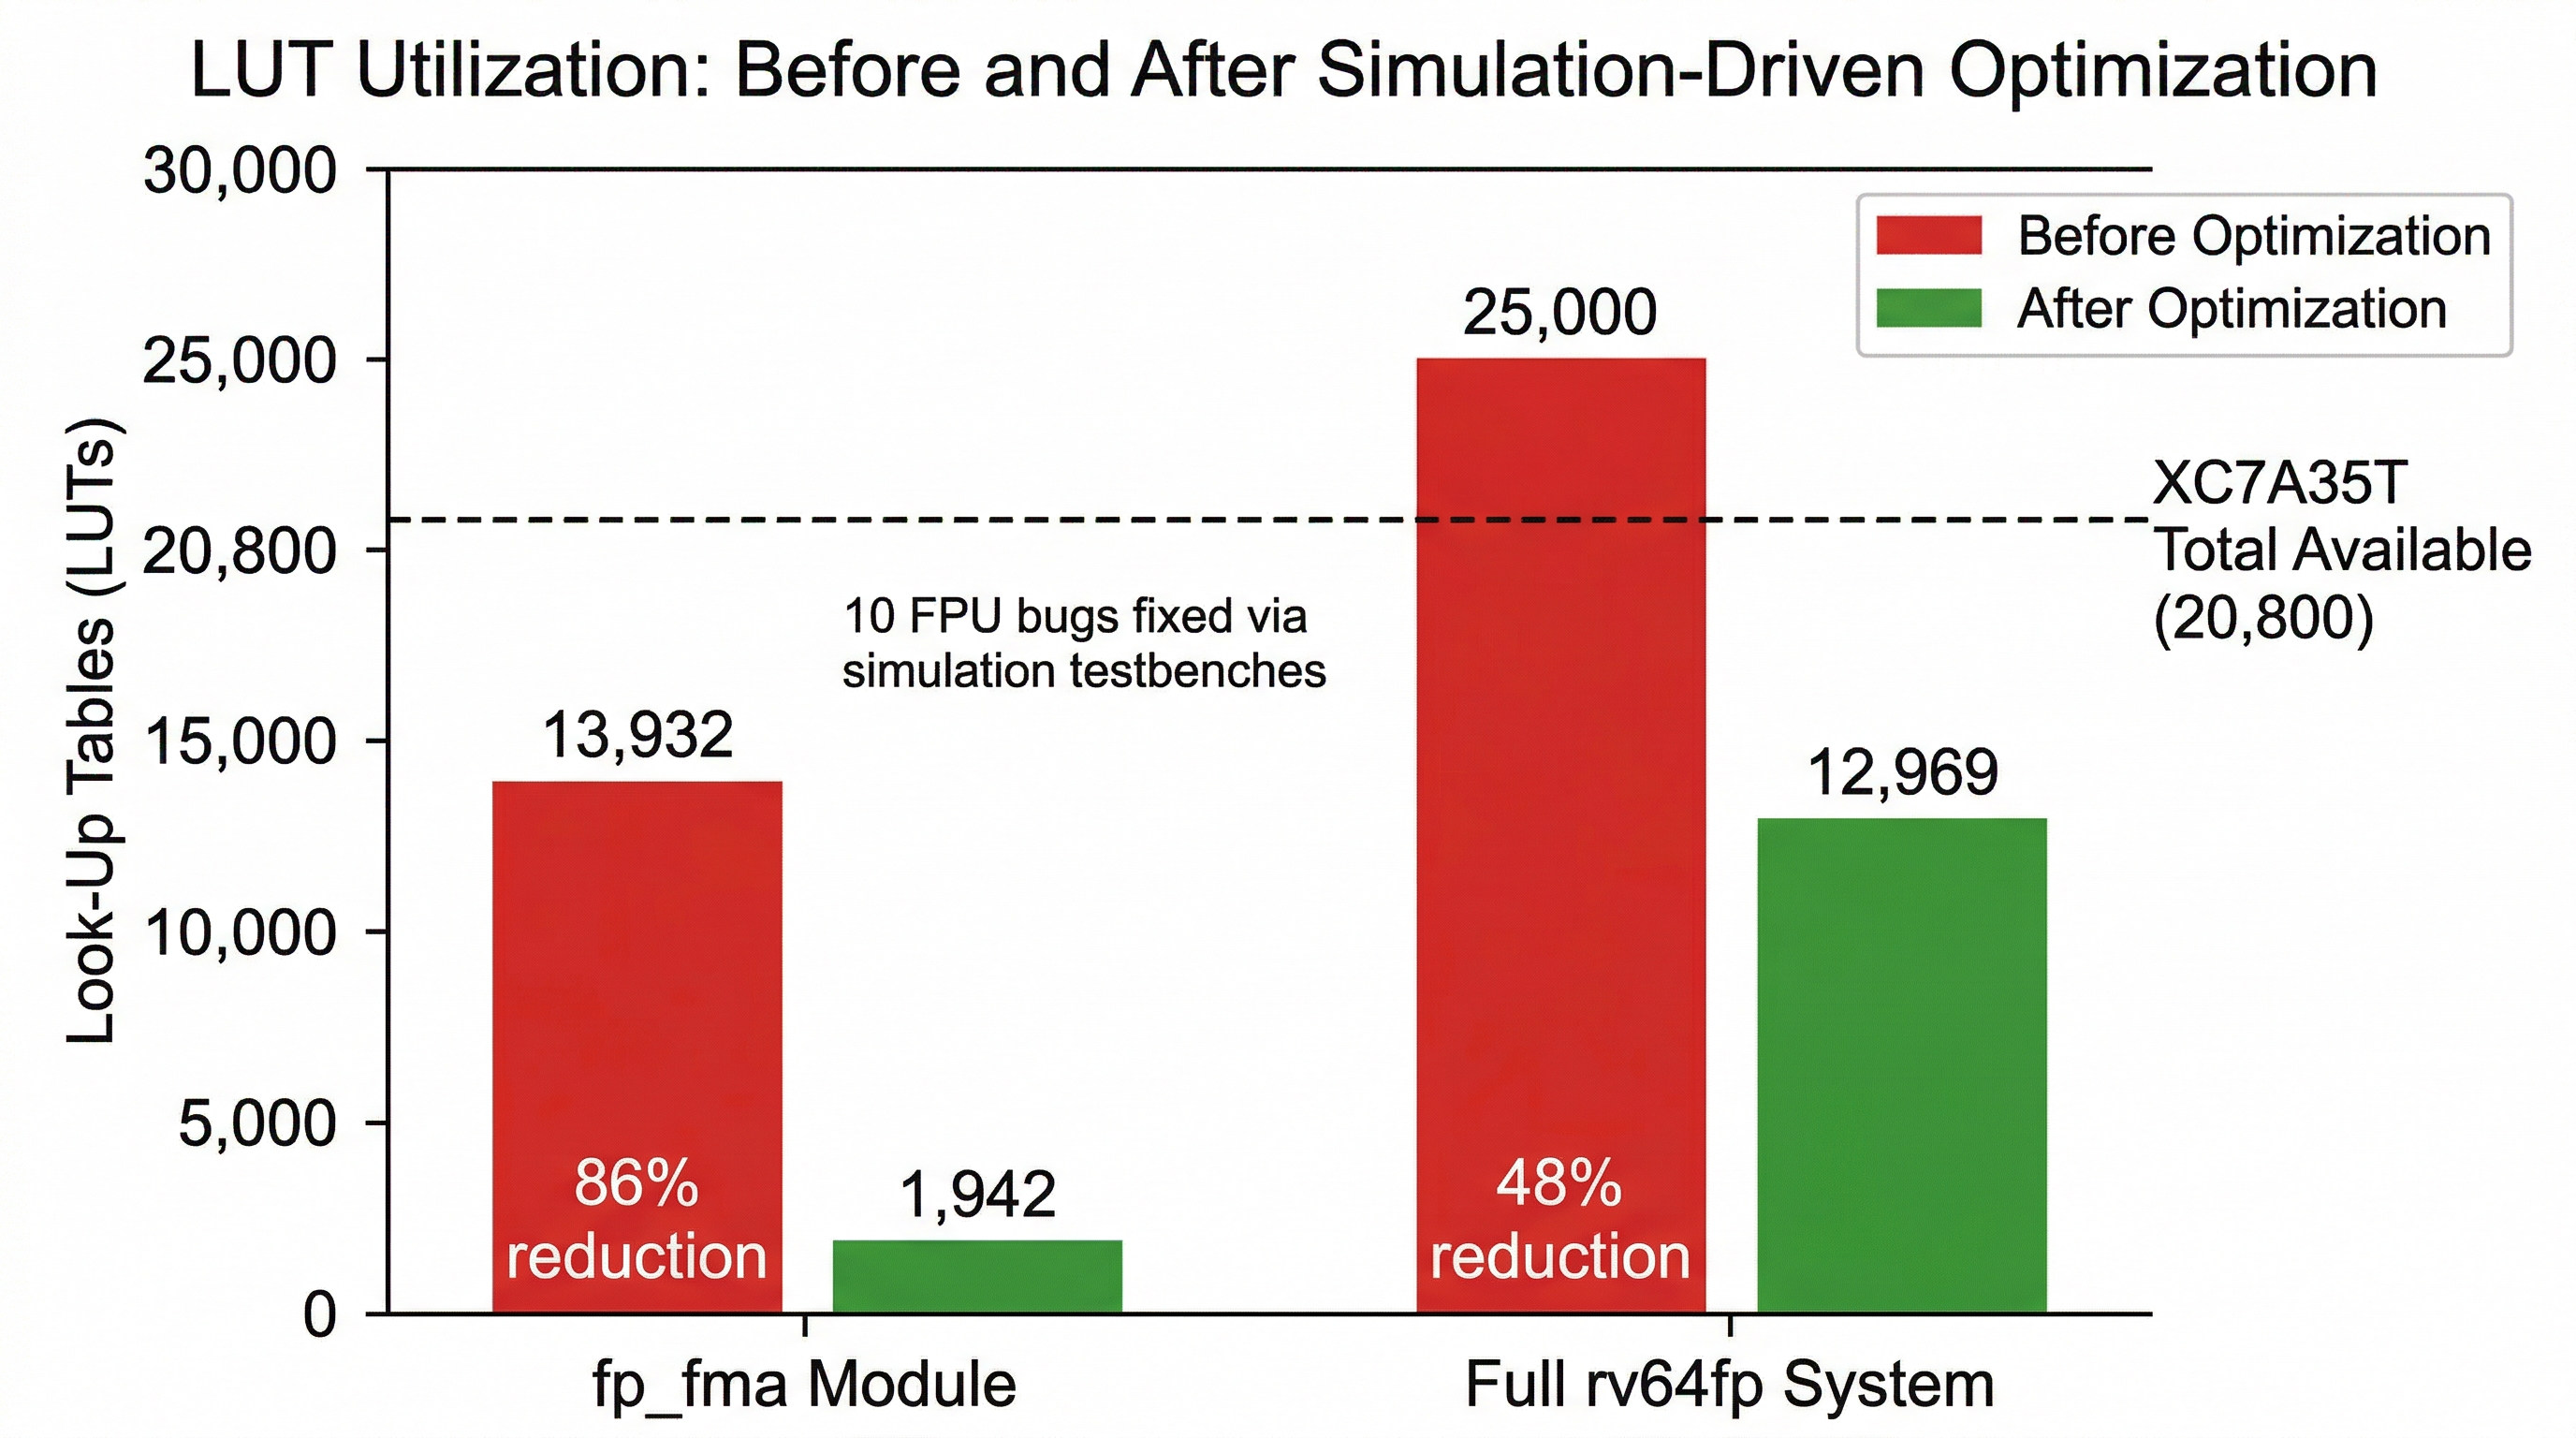
\includegraphics[width=\columnwidth]{figures/fig_lut_optimization.jpg}
  \caption{LUT utilization before and after simulation-driven optimization.}
  \label{fig:lut}
\end{figure}

\subsection{Hardware Verification on Basys 3}

All six processor variants were verified on a Digilent Basys~3 development board~\cite{digilent2021basys3} running at the native 100\,MHz clock frequency under Vivado 2020.2~\cite{xilinx2020ug901}. Hardware verification employed the memory-mapped GPIO interface. Test programs executed on each processor and wrote results to the LED output register, where each of the 16 LED bits represented the pass/fail status of a specific test covering ALU operations, branch instructions, load/store behavior, and individual FPU operations.

This deliberately simple verification strategy was enabled by the exhaustive simulation coverage. The simulation testbenches verified functional correctness comprehensively, so the hardware test served to confirm that the synthesized netlist behaved identically to the simulation model. No discrepancies were observed between simulation and hardware behavior for any of the six designs.

% ─────────────────────────────────────────────────────────────────────
% V. DISCUSSION
% ─────────────────────────────────────────────────────────────────────
\section{Discussion}

The results demonstrate that skill-based context engineering can substantially improve the quality of AI-generated HDL. Without the custom skill, the language model would produce generic Verilog with no simulation infrastructure, no version awareness, and no systematic approach to IEEE 754 special cases. The skill encoded domain expertise that the base model does not possess: patterns for clock-domain crossing, pipeline design with forwarding, BRAM inference rules, and DSP48E1 utilization strategies specific to the Xilinx 7-series architecture~\cite{xilinx2020ds180}.

The simulation-first TDD mandate proved to be the most impactful component of the skill architecture. The 10 bugs caught in the initial FPU generation would have been substantially more expensive to diagnose after synthesis. More significantly, the simulation process drove a 48\% reduction in LUT utilization by revealing that large portions of the generated logic were unreachable or redundant. This finding suggests that AI-generated HDL may systematically over-provision exception handling logic when not constrained by concrete test cases.

The Context7 MCP integration addressed a specific failure mode of LLM-based code generation: confident but incorrect specification of precise technical details. RISC-V instruction encodings require exact bit-field values; a single incorrect bit in the funct7 field produces a different instruction entirely~\cite{waterman2019riscv}. IEEE 754 special-case rules are notoriously subtle: the distinction between quiet NaN and signaling NaN, the sign of zero in subtraction, and the behavior of infinity in division all have precise specifications that the model's training data may not capture accurately~\cite{ieee754_2019}. Live documentation retrieval eliminated this class of errors.

Several limitations of the proposed approach should be noted. First, while formal verification using SVA and bounded model checking has been integrated to prove key correctness properties, the formal proofs are bounded to finite depths (up to 120 cycles for FPU operations) and do not constitute unbounded proofs of correctness. Full induction proofs for the complete processor state space remain computationally intractable for 64-bit datapath designs. Second, the designs operate at the native 100\,MHz clock of the Basys~3 board, but timing closure at higher frequencies has not been attempted. Third, while the 48\% resource optimization is substantial, comparison with manually optimized designs by experienced engineers was not performed.

The integration of formal verification alongside simulation-based testing demonstrates the value of a multi-modal verification strategy for AI-generated HDL. Simulation excels at rapid functional debugging and regression testing, while formal methods provide mathematical guarantees about protocol adherence and invariant preservation. The \texttt{bind} methodology keeps formal verification infrastructure completely separate from the generated RTL, allowing either verification approach to be used independently without modifying the designs. This separation is particularly valuable in the context of AI-generated code, where regeneration may overwrite manual modifications.

% ─────────────────────────────────────────────────────────────────────
% VI. CONCLUSION
% ─────────────────────────────────────────────────────────────────────
\section{Conclusion}

This paper presented a skill-based methodology for AI-assisted RISC-V processor design that produced six complete, hardware-verified processor variants in a single generation session. The custom FPGA skill, constructed by merging community-contributed design knowledge with simulation-first TDD, formal verification via SystemVerilog Assertions, live documentation retrieval, and Vivado version awareness, enabled one-shot generation of designs ranging from a 12-instruction educational core to a 68-instruction RV64IFD processor with a full IEEE 754 double-precision floating-point unit.

The simulation-first verification framework identified 10 FPU bugs in the initial generation and drove a 48\% reduction in LUT utilization, from approximately 25,000 to 12,969 LUTs. Formal verification subsequently proved correctness properties across six categories using SymbiYosys bounded model checking, confirming protocol compliance, ALU and FPU functional correctness, and pipeline hazard detection. The most complex design consumes 82.9\% of the available LUTs on the Xilinx Artix-7 XC7A35T and was verified on a Digilent Basys~3 development board at 100\,MHz. The dual-language output comprises 26 RTL modules per language, totaling 5,721 lines of Verilog and 4,133 lines of VHDL.

Future work will focus on two directions. First, unbounded induction proofs will be pursued for critical properties, potentially using abstract models or assume-guarantee decomposition to manage the 64-bit state space. Second, the approach will be extended to more complex designs including multi-core processors, cache hierarchies, and high-speed serial interfaces to establish the boundaries of skill-based AI-assisted hardware design.

\clearpage
\bibliographystyle{IEEEtran}
\bibliography{references}

\end{document}
